\chapter{Περιγραφή Πλαισίου Έργου}
\section{Πληροφορίες Πελάτη - Mission Statement}
Ο πελάτης-επιχείρηση στον τομέα της παροχής καταλυμάτων ο οποίος επιλέχθηκε είναι το Balance Hotel
Chania. Πρόκειται για μία μικρή, "οικογενειακή" επιχείρηση, η οποία εδρεύει στην πόλη των Χανίων, στην
περιοχή της Νέας Χώρας. Η επιχείρηση δουλεύει καθ'όλη τη διάρκεια ενός ημερολογιακού έτους, 
συναντώντας περισσότερη κίνηση κατά τους θερινούς μήνες. Κατά την θερινή σεζόν λοιπόν, όπου και
συναντάται πιο εύκολα πληρότητα στις κρατήσεις, μπορεί να φιλοξενήσει μέχρι και δεκαεννέα άτομα σε 
εννέα δωμάτια.\\ 

\noindent
Η "αποστολή" της επιχείρησης είναι  να προσφέρει μια bed and breakfast διαμονή σε προσιτές τιμές, 
κοντά στο κέντρο της πόλης, αρκετά μακριά ωστόσο από τα πολυσύχναστα σοκάκια της Παλιάς Πόλης 
ώστε να αποφευχθεί η ενόχληση των πελατών της. Παρέχει ανέσεις που συμπεριλαμβάνονται στα 
περισσότερα καταλύματα της κατηγορίας του, όπως τζακούζι, ανοιχτή ταράτσα, καθημερινό πρωινό, 
ποδήλατα για μετακίνηση μέσα στην πόλη, πάρκινγκ για τους πελάτες. Ακόμα, εντός των δωματίων 
έχουν τοποθετηθεί έξυπνες λάμπες, έξυπνοι θερμοστάτες, smart tv και tablet για χρήση των πελατών
ώστε να είναι εύκολη και ευχάριστη η διαμονή τους. \\

\noindent
Όσον αφορά το προσωπικό της επιχείρησης, σε πλήρη σεζόν απασχολεί πέντε άτομα, ενώ παράλληλα 
εργάζεται και ο ιδιοκτήτης. Βάση αυτής της γνώσης καθώς και των βασικών αλληλεπιδράσεων μεταξύ 
των μελών του προσωπικού, κατασκευάστηκε το οργανωτικό διάγραμμα της επιχείρησης όπως αυτό φαίνεται στο σχήμα \ref{organ_diag} 
\begin{figure}[H]
	\centering
	 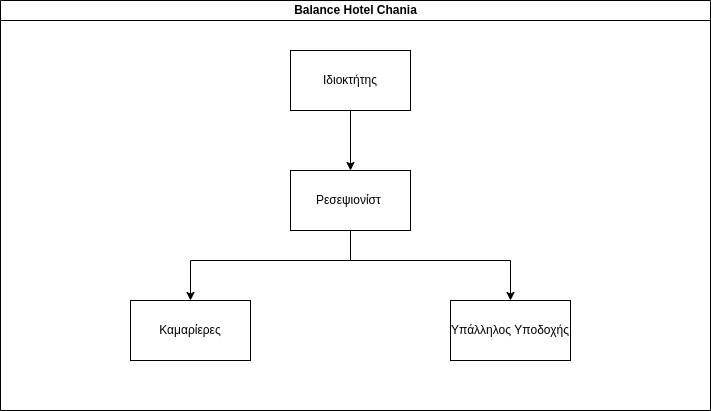
\includegraphics[width=0.9\textwidth]{Images/organization_diagram_2.1}
	 \caption{Organization Diagram}
	\label{organ_diag}
\end{figure}


\section{Περιγραφή Τρέχοντος Συστήματος Πελάτη}
Το τρέχον σύστημα του πελάτη χαρακτηρίζεται από 2 βασικές διεργασίες στην παρούσα φάση. Η πρώτη
αφορά τη δέσμευση των απαραίτητων στοιχείων του πελάτη κατά την δημιουργία νέας κράτησης όπως 
για παράδειγμα όνομα, επώνυμο, ημερομηνία διαμονής και χώρα προέλευσης (πληροφορία που έγινε 
απαραίτητη λόγου του COVID-19) και η  δεύτερη  αφορά την ενημέρωση των προϊόντων που πρέπει να 
προμηθευτεί η επιχείρηση. Όσον αφορά την δεύτερη διαδικασία, κάθε μία από τις καμαριέρες σε 
συνεργασία με τον υπάλληλο υποδοχής καταγράφουν σε ένα αρχείο Excel τα προϊόντα που χρειάζονται 
και στη συνέχεια γίνονται οι αντίστοιχες παραγγελίες στους συνεργαζόμενους  προμηθευτές, μετά από 
τηλεφωνική επικοινωνία.

\section{Αρχιτεκτονική και Πλατφόρμα Τρέχοντος Συστήματος}
\noindent
Οι υποδομές του τρέχοντος συστήματος χωρίζονται στις παρακάτω κατηγορίες:
\begin{itemize}
	\item Hardware
	\item Software
\end{itemize}
	
\noindent
Ως προς το Hardware, κάθε δωμάτιο παρέχει μία συσκευή τηλεφώνου καθώς και μία συσκευή tablet. Ο
υπάλληλος υποδοχής έχει στην διάθεσή του ηλεκτρονικό υπολογιστή βασικών δυνατοτήτων.\\
	
\noindent
Ως προς το software, στον υπολογιστή της υποδοχής γίνεται χρήση λειτουργικού συστήματος Microsoft 
Windows και όσον αφορά τις εφαρμογές, κατά κύριο λόγο γίνεται χρήση του προγράμματος "Microsoft 
Excel" για την καταγραφή των κρατήσεων και των αντικειμένων προς αναπλήρωση. Ακόμα, γίνεται χρήση 
ήδη  υπαρχόντων Mail-server για το Email της επιχείρησης αλλά και έτοιμες πλατφόρμες για τις 
κρατήσεις  Booking, Expedia). Τέλος, τα παρεχόμενα τάμπλετ χρησιμοποιούν λειτουργικό Android και σε 
αυτά  υπάρχουν προεγκατεστημένες οι εφαρμογές με τις πληροφορίες και προτεινόμενες επιχειρήσεις 
καθώς και εφαρμογές για παραγγελία φαγητού.\\


\section{Πλεονεκτήματα, Αδυναμίες, Ευκαιρίες και Απειλές}
Την παρούσα στιγμή, το ξενοδοχείο δεν χρησιμοποιεί κάποιο ψηφιοποιημένο σύστημα για την απογραφή 
των δωματίων ενώ παράλληλα η χρήση των tablets κάθε δωματίου περιορίζεται στις απολύτως  
απαραίτητες λειτουργίες όπως το browsing. \\ 
	
\noindent	
Όσον αφορά στα tablets, είναι σαφές πως δεν έχουν αξιοποιηθεί στο έπακρο και δεν διαδραματίζουν
κάποιο σημαντικό ρόλο στην καθημερινότητα των πελατών. Συνεπώς, το μοναδικό ίσως πλεονέκτημα του
τρέχοντος «συστήματος», όπου ο πελάτης για να κάνει χρήση μίας από τις υπηρεσίες του καταλύματος
πρέπει να έρθει σε επαφή με τον υπάλληλο του ξενοδοχείου είτε μέσω τηλεφώνου είτε με φυσική 
παρουσία στην υποδοχή, είναι η διαπροσωπική σχέση που αναπτύσσεται. Παρόλα αυτά, ο πελάτης 
αναγκάζεται να προβεί σε ενέργειες που δυνητικά μπορεί να του δυσχεραίνουν την διαμονή και την 
χαλάρωσή του. Ακόμη, δεν υπάρχει επαρκής και άμεση ενημέρωση για όλες τις προσφερόμενες υπηρεσίες 
και δραστηριότητες τόσο από το ίδιο το ξενοδοχείο αλλά και από άλλες συνεργαζόμενες επιχειρήσεις 
ενώ ταυτόχρονα, ο πελάτης δεν μπορεί να γνωρίζει σε πραγματικό χρόνο την διαθεσιμότητα των 
φαγητών, των αναψυκτικών και των ποτών που είναι διαθέσιμα προς κατανάλωση στο δωμάτιο. 
Κάνοντας χρήση των tablet για την παροχή τέτοιου είδους πληροφοριών, η διαμονή του πελάτη θα 
γίνεται πιο ευχάριστη καθώς ανά πάσα στιγμή θα έχει πρόσβαση σε πληθώρα πληροφοριών που θα 
μπορεί να αξιοποιήσει για να εμπλουτίσει τις δραστηριότητές του κατά τη διάρκεια της ημέρας ενώ κατά 
την παραμονή του στο δωμάτιο θα είναι σε θέση να γνωρίζει για τα προϊόντα που προσφέρονται. 
Μάλιστα, το πιθανότερο είναι πως το ξενοδοχείο θα παρατηρήσει αύξηση στην κατανάλωση των 
προϊόντων του το οποίο θα επιφέρει αυξήσει κερδών. Ωστόσο, δεδομένου πως ένα τέτοιο σύστημα θα 
μείωνε αισθητά την δια ζώσης επικοινωνία μεταξύ πελάτη και υπαλλήλου ελλοχεύει ο κίνδυνος το 
στοιχείο της ελληνικής φιλοξενίας να μην είναι τόσο έντονο και η διαμονή να γίνει αρκετά απρόσωπη.\\
	
\noindent
Όσον αφορά στην απογραφή των δωματίων, έπειτα από την αποχώρηση του πελάτη το τρέχον 
πρωτόκολλο που ακολουθείται προβλέπει έναν υπάλληλο καθαριότητας (καμαριέρα) μετά τον καθαρισμό 
του δωματίου να αναφέρει, στον υπεύθυνο υποδοχής, τα όποια κλινοσκεπάσματα, κουβέρτες κλπ. 
απουσιάζουν από αυτό. Το συγκεκριμένο μοντέλο δεν παρουσιάζει κάποιο ουσιαστικό πλεονέκτημα ενώ 
διακρίνονται διάφορα μειονεκτήματα δεδομένου πως βασίζεται στον ανθρώπινο παράγοντα. Είναι 
ιδιαίτερα πιθανό να υπάρχουν παραλήψεις κατά την απογραφή, τόσο από την καμαριέρα όσο και από την 
υπεύθυνη, καθώς όλη η διαδικασία της καταγραφής γίνεται με χρήση προφορικού λόγο όπου η καμαριέρα 
αναφέρει τα αντικείμενα που απουσιάζουν και γίνεται η καταγραφή τους από την υπεύθυνη. Ακόμα, 
υπάρχει η περίπτωση η καμαριέρα να μην γνώριζε εξαρχής την ύπαρξη κάποιου αντικειμένου. Τέλος, δεν 
υπάρχει κάποιος εύκολος και γρήγορος τρόπος ανά πάσα στιγμή να γνωρίζει ο ιδιοκτήτης τον αριθμό των 
χαμένων αντικειμένων το οποίο μεταφράζεται σε κόστος για την επιχείρηση. Συνεπώς, με τον τρόπο 
αυτό θα μπορέσει και το ξενοδοχείο να κάνει καλύτερη διαχείριση των πόρων που καταναλώνονται.


\section{Εμβέλεια Έργου και Περιορισμοί Κύκλου Έργου}		
Το σύστημα έχει σκοπό να διαχειρίζεται την επικοινωνία μεταξύ υποδοχής και πελάτη κατά την διάρκεια 
της διαμονής του ενώ παράλληλα να αυξήσει την αποδοτικότητα και την ταχύτητα βασικών εργασιών 
που συμβαίνουν στα δωμάτια σε τακτά χρονικά διαστήματα.\\

\noindent
Αρχικά, μέσω του υλοποιούμενου συστήματος ο πελάτης θα έχει την δυνατότητα αλληλεπίδρασης, σε 
πραγματικό χρόνο, με τον υπεύθυνο του καταλύματος με σκοπό να δεχτεί υπηρεσίες δωματίου όπως το 
πρωινό στο δωμάτιο σε συγκεκριμένο ώρα ή την παραγγελία κάποιου άλλου γεύματος ή ποτού ενώ θα 
ενημερώνεται σε πραγματικό χρόνο για την επιβεβαίωση ή την απόρριψη του αιτήματος.  Ακόμα, θα 
δίνεται η δυνατότητα εύρεσης αξιοθέατων της πόλης ή επιχειρήσεων όπως εστιατόρια, μαγαζιά με 
ζωντανή μουσική αλλά και εταιρείες ενοικίασης οχημάτων, σύμφωνα με προτάσεις του ξενοδοχείου. Οι 
πιο συνηθισμένες ερωτήσεις θα βρίσκονται σε μορφή FAQ (Frequently Asked Questions) μαζί με τις 
απαντήσεις τους. Τέλος, θα δίνεται η δυνατότητα επικοινωνίας, μέσω της εφαρμογής, με την υποδοχής 
και πιο συγκεκριμένα με τον υπάλληλο που δουλεύει εκείνη την ώρα, στην περίπτωση που ο πελάτης 
επιθυμεί να επικοινωνήσει με αυτή. Οι απαντήσεις εμφανίζονται και αυτές στον πελάτη μέσω της 
εφαρμογής. \\

\noindent
Όσον αφορά τις λειτουργίες που θα αφορούν για τους υπαλλήλους, θα δίνεται η δυνατότητα στους 
υπάλληλους του προσωπικό καθαριότητας να αναφέρουν τον αριθμό των δωματίων που ανέλαβαν 
καθώς και τον αριθμό των αντικειμένων που λείπουν από κάθε δωμάτιο, σε περίπτωση που συμβεί αυτό, 
ώστε να μπορούν να αναπληρωθούν άμεσα εφόσον έχει τελειώσει η διαμονή του προηγούμενου πελάτη. 
\\

\noindent
(Αυτή τη στιγμή, η γενικότερη επικοινωνία με τον υπεύθυνο υποδοχής γίνεται είτε μέσω τηλεφώνου που 
διαθέτει κάθε δωμάτιο είτε μέσω εφαρμογών κοινωνικής δικτύωσης (ενδεικτικά Viber, Whatsapp). 
Ειδικότερα, στις περιπτώσεις που δεν χρησιμοποιείται το τηλέφωνο δωματίου, πιθανώς η επικοινωνία 
να μην είναι πάντα άμεση καθώς ο υπάλληλος με τον οποίο επικοινωνούν να βρίσκεται εκτός ωραρίου. 
Αυτό  αρχικά θεωρείται αντιεπαγγελματικό και ταυτόχρονα αποθαρρυντικό για τον πελάτη καθώς μία 
απάντηση μπορεί να σταλεί μετά από αρκετές ώρες (όταν είναι και πάλι η βάρδια του συγκεκριμένου 
υπαλλήλου). Όσον αφορά την απογραφή, γίνεται σε ένα αρχείο Excel το οποίο το  διαχειρίζεται ο 
υπεύθυνος υποδοχής και αποτελεί μία αρκετά χρονοβόρα διαδικασία.) \\

\noindent
Σε σχέση με τις επιθυμίες του πελάτη, το σύστημα υπερκαλύπτει τις αρχικές απαιτήσεις δηλαδή την 
βελτίωση της επικοινωνίας μεταξύ υποδοχής και πελατών αλλά και την αξιοποίηση των tablet που μέχρι 
στιγμής δεν χρησιμοποιούνται ουσιαστικά. Ταυτόχρονα, χρονοβόρες διαδικασίες όπως αυτή της 
καταμέτρησης των δωματίων που καθαρίστηκαν και των απωλειών που προέκυψαν θα γίνονται με πολύ πιο 
αποδοτικό τρόπο. \\

\noindent
Κατά την υλοποίηση ενδεχομένως προκύψουν προβλήματα ως προς την ταχύτητα απόκρισης του συστήματος 
καθώς είναι απαραίτητο η επικοινωνία να είναι άμεση και απροβλημάτιστη. Για την εξασφάλιση της ομαλής 
λειτουργίας πιθανώς να απαιτείται αναβάθμιση των πληροφοριακών συστημάτων του καταλύματος 
(υπολογιστές, βάση δεδομένων) ή/και χορήγηση κινητών τηλεφώνων νέας γενιάς στους υπαλλήλους που δεν 
διαθέτουν ώστε  να μπορούν να διαχειρίζονται το σύστημα μέσω της αντίστοιχης εφαρμογής. Παρόλο το 
μικρό μέγεθος της επιχείρησης, το χρονικό κόστος υλοποίησης ενδέχεται να αυξηθεί κατά (χρόνος) 
συμπεριλαμβανομένου των εργασιών εγκατάστασης, ώστε το σύστημα να ανταποκρίνεται στις προδιαγραφές.
Ακόμα, είναι απαραίτητο να δοθεί ιδιαίτερη έμφαση στην δημιουργία ενός εύχρηστου γραφικού 
περιβάλλοντος ώστε η χρήση της εφαρμογής να μην απαιτεί ιδιαίτερες τεχνικές γνώσεις και ως αποτέλεσμα 
κάθε διαδικασία να γίνεται εύκολα και χωρίς να δυσκολεύει τους χρήστες. Μία τέτοια εφαρμογή, απαιτεί 
από τον ομάδα που την υλοποιεί, βασικές γνώσεις προγραμματισμού πάνω στις εφαρμογές κινητών αλλά και 
υπολογιστών ενώ ταυτόχρονα αυξάνει αρκετά τον απαιτούμενο χρόνο υλοποίησης. Ενδεικτικά, μία 
αντίστοιχη εφαρμογή  απαιτεί (χρόνο) για την δημιουργία της.\\ 

\noindent
Προς αποφυγή των παραπάνω εξόδων, είναι απαραίτητο να δοθεί ιδιαίτερη προσοχή στις απαιτήσεις υλικών 
πόρων (Hardware) ώστε να μην είναι μεγάλες. Ακόμα, σημαντικό είναι τα άτομα που θα αναλάβουν την 
δημιουργία των εφαρμογών να έχουν τις απαραίτητες γνώσεις αλλά και εμπειρία πάνω στον τομέα του. 
Επίσης, για να υπάρχει το καλύτερο δυνατό αποτέλεσμα είναι σημαντικό ο ιδιοκτήτης του καταλύματος 
αλλά και οι υπάλληλοι να έχουν την δυνατότητα δοκιμής της εφαρμογής ώστε να παρέχουν το κατάλληλο 
feedback ώστε το τελικά προϊόν να είναι το καλύτερο πιθανό. Τέλος, κάθε πιθανή καθυστέρηση ενώ δεν 
εμποδίζει την λειτουργία του καταλύματος, δεν συμβάλει και στην βελτίωσή του κάτι το οποίο μπορεί να 
θεωρηθεί ως κόστος.
		
		
		    